\documentclass[2pt,a4paper]{article}
\usepackage[utf8]{inputenc}
\usepackage[french]{babel}
\usepackage[T1]{fontenc}
\usepackage{amsmath}
\usepackage{amsfonts}
\usepackage{amssymb}
\usepackage{graphicx}
\usepackage{epstopdf}
\usepackage{lmodern}
\usepackage{eurosym}
\usepackage{textcomp}
\usepackage{subfigure}
\usepackage{placeins}
\usepackage{listings}
\usepackage{proof}
\usepackage{amsthm}
\usepackage[left=1cm,right=1cm,top=2cm,bottom=1cm]{geometry}
\usepackage{color}
\usepackage{multicol}
\usepackage{fancyhdr}
\usepackage{tikz}

\tikzstyle{vertex}=[circle,fill=gray!50,minimum size=15pt,inner sep=0pt]
\tikzstyle{visited}=[circle,fill=green!25,minimum size=15pt,inner sep=0pt]
\tikzstyle{unvisited}=[circle,fill=blue!25,minimum size=15pt,inner sep=0pt]

\newcommand{\W}{\ {\color{red} \textbf{!!}} \ }

\setlength{\headsep}{0.2in}
\definecolor{listinggray}{gray}{0.9}
\definecolor{lbcolor}{rgb}{0.9,0.9,0.9}
\definecolor{mygreen}{rgb}{0,0.6,0}
\definecolor{mygray}{rgb}{0.5,0.5,0.5}
\definecolor{mymauve}{rgb}{0.58,0,0.82}

\pagestyle{fancy}
\fancyhf{}
\renewcommand{\sectionmark}[1]{\markright{#1}}
\fancyhead[RO]{\textbf{\thepage}}
\fancyhead[LO]{Université Catholique de Louvain}
%\fancyhead[RE]{\textsl{\leftmark}}
\renewcommand{\headrulewidth}{1px}

\lstset{ %
  backgroundcolor=\color{white},
  basicstyle=\footnotesize,
  breakatwhitespace=false,
  breaklines=true,
  captionpos=b,
  commentstyle=\color{mygreen},
  deletekeywords={},
  escapeinside={\%*}{*)},
  extendedchars=true,
  frame=none,
  keepspaces=true,
  keywordstyle=\color{blue},
  language=Java,
  morekeywords={},
  numbers=none,
  numbersep=0pt,
  numberstyle=\tiny\color{mygray},
  rulecolor=\color{black},
  showspaces=false,
  showstringspaces=false,
  showtabs=false,
  stepnumber=0,
  stringstyle=\color{mymauve},
  tabsize=2,
  belowskip=0pt,
  aboveskip=0pt,
}
\setlength{\parindent}{0cm}
\setlength{\columnseprule}{1px}
\author{François Aubry, Guillaume Derval, Benoît Legat, Anthony Gégo}
\title{Formulaire BAPC}
\begin{document}
\begin{multicols}{2}
{\Huge Formulaire BAPC 2013}\\
{\Large Team UCooL}\\
Auteurs: François Aubry, Guillaume Derval, Benoît Legat, Anthony Gégo.
\tableofcontents
\section{Remarques}
\subsection{Attention!}
\begin{enumerate}
	\item Lire \textbf{TOUS} les énoncés avant de commencer la moindre implémentation
	\item Faire attention au copier-coller bête et méchant.
	\item Surveiller les overflow. Parfois, un long peux régler pas mal de problèmes
\end{enumerate}
 
\subsection{Opérations sur les bits}
\begin{enumerate}
	\item Vérification parité de $n$: \lstinline{(n & 1) == 0}
	\item $2^n$: \lstinline|1 << n|.
	\item Tester si le $i$ème bit de $n$ est $0$: \lstinline{(n & 1 << i) != 0}
	\item Mettre le $i$ème bit de $n$ à 0: \lstinline{n &= ~(1 << i)}
	\item Mettre le $i$ème bit de $n$ à 1: \lstinline{n |= (1 << i)}
	\item Union: \lstinline{a | b}
	\item Intersection: \lstinline{a & b}
	\item Soustraction bits: \lstinline{a & ~b}
	\item Vérifier si $n$ est une puissance de 2: \lstinline{(x & (x-1) == 0)}
	\item Passage au négatif: \lstinline{0x7fffffff^n}
\end{enumerate}
\section{Graphs}
\subsection{Basics}
\begin{itemize}
\item Adjacency matrix: $A[i][j] = 1$ if $i$ is connected to $j$ and $0$ otherwise
\item Undirected graph: $A[i][j] = A[j][i]\ \forall\ i,j$ ($A = A^T$)
\item Adjacency list: \lstinline|LinkedList<Integer>[] g;|
$g[i]$ stores all neighbors of $i$
\item Useful alternatives: 
\begin{lstlisting}
HashSet<Integer>[] g; // for edge deletion
HashMap<Integer, Integer>[] g; // for weighted graph
\end{lstlisting}
\item Basic classes
\lstinputlisting{graphs/basics.java}
\end{itemize}
\subsection{BFS}
Computes $d$, an array of distance from start vertex $v$.
$d[v]=0$, $d[u]=\infty$ if $u$ not connected to $v$. If $(u, w)\in E$ and $d[u]$ known and $d[w]$ unknown, $d[w] = d[u]+1$.\\
\lstinputlisting{Graphs/bfsvisit.java}
\subsubsection{Connected components}
\lstinputlisting{Graphs/bfs.java}
\subsubsection{Girth}
The girth of an undirected graph is the length of its shortest cycle ($\infty$ if none). Complexity $O(|V| |E|)$. \\

\lstinputlisting{Graphs/girth.java}

\subsection{DFS}
Equals to BFS with \textit{Stack} instead of \textit{Queue} or recursive implementation. Complexity $O(|V|+|E|)$\\
\lstinputlisting{Graphs/dfs.java}
\subsubsection{Topological order}
Graph must be acyclic.
\lstinputlisting{Graphs/toposort.java}
\subsubsection{Strongly connected components}
Uses BFS following the topologic order.
\lstinputlisting{Graphs/scc.java}
\subsection{Minimum Spanning Tree}
\subsubsection{Prim}
\lstinputlisting{Graphs/prim.java}
\subsubsection{Kruskal}
Uses Union-Find (See section \ref{unionFind}).
\lstinputlisting{Graphs/kruskal.java}
\subsection{Dijksta}
Plus court chemin d'un noeud $v$ à tout les autres. Le graphe doit être sans cycles de poids négatif.\\

\begin{lstlisting}
double[] dijkstra(LinkedList<Edge>[] g, int v)
{
  double[] d = new double[g.length];
  Arrays.fill(d, Double.POSITIVE_INFINITY);
  // initialize distance to v and the priority queue
  d[v] = 0;
  PriorityQueue<Edge> PQ = new PriorityQueue<Edge>();
  for(Edge e : g[v])
    PQ.add(e);
  while(!PQ.isEmpty())
  {
    // poll minimum edge from PQ
    Edge minE = PQ.poll();
    if(d[minE.dest] == Double.POSITIVE_INFINITY)
    {
      // set the distance to the new found endpoint
      d[minE.dest] = minE.w;
      for(Edge e : g[minE.dest])
      {
        // add to the queue all edges leaving the new
        // endpoint with the increased weight
        if(d[e.dest] == Double.POSITIVE_INFINITY)
          PQ.add(new Edge(e.orig, e.dest, e.w + d[e.orig]));
      }
    }
  }
  return d;
}
\end{lstlisting}
\subsection{Bellman-Ford\label{BellmanFord}}
Plus court chemin d'un noeud $v$ à tout les autres. Le graphe peut avoir des cycles de poids négatif, mais alors l'algorithme ne retourne pas les chemins les plus courts, mais retourne l'existence de tels cycles.\\
$d[i][u] = \text{shortest path from $v$ to $u$ with $\leq i$ edge}$\\
$d[0][v] = 0$ \\
$d[0][u] = \infty \quad \text{for $u \neq v$}$\\
$d[i][u] = \min \{ 
d[i - 1][u], \quad
\min_{(s, u) \in E} d[i - 1][s] + w(s, u) \}$\\
Si pas de cycle, la solution est dans $d[|V|-1]$. Si cycle il y a, $d[|V|-1]=d[V]$.\\
$O(|V||E|)$.\\

\begin{lstlisting}
static double[] bellmanFord(LinkedList<Edge> gt, int v, int n) {
  double[] dist = new double[n];
  Arrays.fill(dist, Double.POSITIVE_INFINITY);
  dist[v] = 0;
  for(int i=0; i < n-1; i++)
    for(Edge e : gt)
      if(dist[e.o] + e.w < dist[e.d])
        dist[e.d] = dist[e.o] + e.w;
  for(Edge e : gt)
    if(dist[e.o] + e.w < dist[e.d])
      return null;
  return dist;
}
\end{lstlisting}
\begin{lstlisting}
static double[] spfa (LinkedList<Edge>[] g, int s) {
  int n = g.length;
  double[] dist = new double[n];
  Arrays.fill(dist, Double.POSITIVE_INFINITY);
  Queue<Integer> q = new LinkedList<Integer>();
  BitSet inQueue = new BitSet(n);
  int[] timesIn = new int[n];

  dist[s] = 0;
  q.add(s);
  inQueue.set(s);
  timesIn[s]++;
  while (!q.isEmpty()) {
    int cur = q.poll(); inQueue.clear(cur);
    for (Edge next : g[cur]) {
      int v = next.d, w = next.w;
      if (dist[cur] + w < dist[v]) {
        dist[v] = dist[cur] + w;
        if (!inQueue.get(v)) {
          q.add(v);
          inQueue.set(v);
          timesIn[v]++;
          if (timesIn[v] >= n) {
            return null; // Infinite loop
          }
        }
      }
    }
  }
  return dist;
 }
\end{lstlisting}
\subsection{Floyd-Warshall}
Plus court chemin de tout les noeuds à tout les autres. Prend en argument la matrice d'adjacence. $O(|V|^3)$ en temps et $O(|V|^2)$ en mémoire.\\
Le graphe contient des cycles de poids négatif ssi $result[v][v]<0$.\\

\begin{lstlisting}
double[][] floydWarshall(double[][] A)
{
  int n = A.length;
  // initialization: base case
  double[][] d = new double[n][n];
  for(int v = 0; v < n; v++)
    for(int u = 0; u < n; u++)
      d[v][u] = A[v][u];

  for(int k = 0; k < n; k++)
    for(int v = 0; v < n; v++)
      for(int u = 0; u < n; u++)
        d[v][u] = Math.min(d[v][u], d[v][k] + d[k][u]);
  return d;
}
\end{lstlisting}

\subsection{Max flow}
\subsubsection{Edmonds-Karps (BFS)}
Path in residual graph searched via BFS. $O(|V||E|^2)$.\\
\lstinputlisting{Graphes/edmondskarps.java}
\subsubsection{Ford-Fulkerson}
Equals to Edmonds-Karps, vut with a DFS. $O(|E|f^*)$ where $f^*$ is the value of the max flow.
\subsubsection{Shorter but slower implementation}
\lstinputlisting{Graphes/maxflowslower.java}
\subsubsection{Min cut}
We search, between two nodes $s$ and $t$, $V_1$ and $V_2$ so as $s\in V_1$, $t\in V_2$ and $\sum_{e \in E(V_1, V_2)} w(e)$ minimum.\\
We just have to compute the max-flow between $s$ and $t$ and to apply a BFS/DFS on the residual graph. All node which are visited are in $V_1$, others in $V_2$. The weight from the cut is the max-flow.
\subsubsection{Maximum weighted bipartite matching}
(Assignment problem)
\lstinputlisting{Graphes/mwbm.java}
\subsection{Bipartite graph}
Check if bipartite
\lstinputlisting{Graphs/isBipartite.java}

\subsubsection{Max Cardinality Bipartite Matching (MCBM)}
Pairing of adjacent nodes. No node in two different pairs.
\begin{itemize}
  \item Max Flow.
  \item Augmenting Path: path starting at non matched, ending
    at non-matched, even edges are matching.
    MCBM ssi no augmenting path.
    Start from non-matched, if augmenting path, augment
    (do not have to take all matching in the augmenting path).
\end{itemize}
MCBM : Number of matching.

Hungarian algorithm $O(|V||E|)$:
\lstinputlisting{Graphs/hungarian.java}

Hopcroft-Karp algorithm $O(\sqrt{|V|}|E|)$:
\lstinputlisting{Graphs/hopcroftkarp.java}

\subsubsection{Independent Set (or Dominating Set)}
Set of vertices with no edges between them.
MIS, add a vertex create an edge.
In \textbf{bipartite} graph,
$\text{MIS} + \text{MCBM} = V$.

\subsubsection{Vertex Cover}
Vertices such that each edge is adjacent to at least one vertex.
Min Vertex Cover (MVC). In \textbf{bipartite} graph,
$\text{MVC} = \text{MCBM}$.

In \textbf{general} graph,
$\text{MIS} + \text{MVC} = |V|$ and the MVC is the complementary of MIS.


\section{Dynamic programming}
\subsection{Bottom-up}
Give n objects of value $v[i]$ to 3 people such that $\max_i V_i - \min_i V_i$ is minimum ($V_i$ is total value for person $i$).

$canDo[i][v_1][v_2]$ =  1 if we can give the objects $0, 1, \ldots, i$ such that $v_1$ is going to $P_1$ and $v_2$ to $P_2$, 0 otherwise. $v_3$ is determined from the sum.

\begin{minipage}{0.25\textwidth}
\textbf{Base case $i = 0$:}
\begin{itemize}
\item $ canDo[0][0][0]  = 1$
\item $ canDo[0][v[0]][0]  = 1$ 
\item $ canDo[0][0][v[0]]  = 1$
\end{itemize}
\end{minipage}
\begin{minipage}{0.25\textwidth}
\textbf{Case $i \geq 1$:} 

$ canDo[i][v_1][v_2] =  \\\text{\ \ }canDo[i - 1][v_1][v_2] \vee \\  \text{\ \ }canDo[i - 1][v_1 - v[i]][v_2] \vee \\  \text{\ \ } canDo[i - 1][v_1][v_2 - v[i]] $
\end{minipage}
\newline
\textbf{Sol. :} $ \min_{v_1, v_2 : canDo[n - 1][v_1][v_2]} \quad [max(v_1, v_2, S - v_1 - v_2) - min(v_1, v_2, S - v_1 - v_2)]$
\newline
\begin{lstlisting}
int solveDP() {
  boolean[][][] canDo = new boolean[v.length][sum + 1][sum + 1];
  // initialize base cases
  canDo[0][0][0] = true;
  canDo[0][v[0]][0] = true;
  canDo[0][0][v[0]] = true;
  // compute solutions using recurrence relation
  for(int i = 1; i < v.length; i++) {
    for(int a = 0; a <= sum; a++) {
      for(int b = 0; b <= sum; b++) {
        boolean giveA = a - v[i] >= 0 && canDo[i - 1][a - v[i]][b];
        boolean giveB = b - v[i] >= 0 && canDo[i - 1][a][b - v[i]];
        boolean giveC = canDo[i - 1][a][b];
        canDo[i][a][b] = giveA || giveB || giveC;
      }
    }
  }
  // compute best solution
  int best = Integer.MAX_VALUE;
  for(int a = 0; a <= sum; a++) {
    for(int b = 0; b <= sum; b++) {
      if(canDo[v.length - 1][a][b]) {
        best = Math.min(best, max(a, b, sum - a - b) - min(a, b, sum - a - b));
      }
    }
  }
  return best;
}
\end{lstlisting}
\subsection{Top-down}
Même problème que bottom-up. Idée principale : mémoisation (On retient les résultats intermédiaires).
\newline
\begin{lstlisting}
int solve(int i, int a, int b) {
  if(i == n) {
    memo[i][a][b] = max(a, b, sum - a - b) - min(a, b, sum - a - b);
    return memo[i][a][b]; 
  }
  if(memo[i][a][b] != null) {
    return memo[i][a][b];
  }
  int giveA = solve(i + 1, a + v[i], b);
  int giveB = solve(i + 1, a, b + v[i]);
  int giveC = solve(i + 1, a, b);
  memo[i][a][b] = min(giveA, giveB, giveC);
  return memo[i][a][b];
}
\end{lstlisting}
\subsection{Problème du sac à dos (Knapsack)}
On a $n$ objets de valeurs $v[i]$ et de poids $w[i]$, un entier $W$, on veut:
\begin{itemize}
\item Maximiser  $\sum_i x[i] v[i]$
\item Avec $\sum_i x[i] w[i] \leq W$ \hspace{15pt} où $ x[i] $= 0 (pas pris) ou 1 (pris)
\end{itemize}
\subsubsection{Un exemplaire de chaque}
best[i][w]= meilleur façon de prendre les objets $0, 1, \ldots, i$ dans sac à dos de capacité $w$.

\begin{minipage}{0.25\textwidth}
\textbf{Cas de base:}
\begin{itemize}
\item $best[0][w] = v[0]$ \\si $w[0] \leq w$
\item 0 sinon
\end{itemize}
\end{minipage}
\begin{minipage}{0.25\textwidth}
\textbf{Autres cas:}\\
$best[i][w]   = \\ \text{\ \ }\max \{ best[i-1][w], \\ \text{\ \ \ \ }best[i-1][w-w[i]] + v[i] \}$
\end{minipage}
\subsubsection{Plusieurs exemplaires de chaque}
\begin{itemize}
\item $ best[0] = 0$
\item $best[w] = \max_{i : w[i] < w} \{best[w - w[i]] + v[i]\}$
\end{itemize}

\subsubsection{Plusieurs knapsack}

$best[i][w_1][w_2] =$ meilleur façon de prendre les objets $0, 1, \ldots, i$ dans des sacs de capacités $w_1$ et $w_2$.
\subsection{Longest common sub-sequence (LCS)}
Given two String $x$ and $y$. Find the longest common sub-sequence between $x$ and $y$.
 
\begin{center}
\begin{tikzpicture}[scale = 0.7]
\node at (-1, 1) {$x$};
\node at (-1, 0) {$y$};

\node[draw, circle] at (0, 0) (A)                  {\tiny G};
\node[draw, circle, fill = blue!25] at (1, 0) (B)  {\tiny C};
\node[draw, circle, fill = blue!25] at (2, 0) (C)  {\tiny A};
\node[draw, circle, fill = blue!25] at (3, 0) (D)  {\tiny A};
\node[draw, circle, fill = blue!25] at (4, 0) (E)  {\tiny G};
\node[draw, circle, fill = blue!25] at (5, 0) (F)  {\tiny T};
\node[draw, circle] at (6, 0) (G)                  {\tiny C};
\node[draw, circle, fill = blue!25] at (7, 0) (H)  {\tiny T};
\node[draw, circle, fill = blue!25] at (8, 0) (I)  {\tiny A};
\node[draw, circle, fill = blue!25] at (9, 0) (J)  {\tiny A};
\node[draw, circle, fill = blue!25] at (10, 0) (K) {\tiny T};
\node[draw, circle, fill = blue!25] at (11, 0) (L) {\tiny A};

\node[draw, circle, fill = blue!25] at (0, 1) (a)  {\tiny C};
\node[draw, circle, fill = blue!25] at (1, 1) (b)  {\tiny A};
\node[draw, circle, fill = blue!25] at (2, 1) (c)  {\tiny A};
\node[draw, circle] at (3, 1) (d)                  {\tiny G};
\node[draw, circle, fill = blue!25] at (4, 1) (e)  {\tiny G};
\node[draw, circle, fill = blue!25] at (5, 1) (f)  {\tiny T};
\node[draw, circle, fill = blue!25] at (6, 1) (g)  {\tiny T};
\node[draw, circle, fill = blue!25] at (7, 1) (h)  {\tiny A};
\node[draw, circle] at (8, 1) (i)  {\tiny T};
\node[draw, circle, fill = blue!25] at (9, 1) (j)  {\tiny A};
\node[draw, circle, fill = blue!25] at (10, 1) (k) {\tiny T};
\node[draw, circle, fill = blue!25] at (11, 1) (l) {\tiny A};

\draw (B) edge (a);
\draw (C) edge (b);
\draw (D) edge (c);
\draw (F) edge (f);
\draw (H) edge (g);
\draw (I) edge (h);
\draw (K) edge (k);
\draw (L) edge (l);
\draw (E) edge (e);
\draw (J) edge (j);

\end{tikzpicture}
\end{center}

\begin{itemize}
 \item \textbf{Formulation:}
$lcs[i][j] =$ size of \\\text{\ \ \ } $LCS(x[0] x[1] \cdots x[i - 1], y[0] y[1] \cdots y[j - 1])$
  \item \textbf{Base case:} $
lcs[0][j]  = 0$ \hspace{15pt} 
$lcs[i][0]  = 0$
  \item \textbf{Other cases: }
  \begin{itemize}
  \item Si $x[i-1] = y[i-1]$ alors: \\
  \quad $lcs[i][j] = 1 + lcs[i-1][j-1]$ 
  \item Si $x[i-1] \neq y[i-1]$ alors: \\
  \quad $lcs[i][j] = \max \{lcs[i-1][j], lcs[i][j-1]\}$
  \end{itemize}
\end{itemize}
\subsection{Matrix Chain Multiplication (MCM)}
Given a list of matrices, find the order minimizing the number of multiplications to compute their product.
\begin{itemize}
 \item Number to multiply a matrix of size $n \times m$ by a matrix of size $m \times r$ : $n \cdot m \cdot r$.

 \item Example: $A$ : $10 \times 30$, $B$ : $30 \times 5$ et $C$ : $5 \times 60$.
 \begin{itemize}
 \item For $(AB)C$ : $10 \cdot 30 \cdot 5 + 10 \cdot 5 \cdot 60 = 4500$ multiplications.
 \item For $A(BC)$ : $30 \cdot 5 \cdot 60 + 10 \cdot 30 \cdot 60 = 27000$ multiplications.
  \end{itemize}
\end{itemize}

\begin{itemize}
 \item \textbf{Formulation :}
 $best[i][j] =$ min cost to multiply $A_i, \ldots, A_j$
 \item \textbf{Base case :} $best[i][i] = 0 $
 \item \textbf{Other cases:}
 \begin{align*}
 best[i][j] = \min_{i \leq k < j} best[i][k] & + best[k + 1][j] \\
                                             & + A_i.n_1 \times A_k.n_2 \times A_j.n_2
 \end{align*}
\end{itemize}

\subsubsection{Generalized MCM}
Given a list of objects $x[0], \ldots, x[n - 1]$ and an operation $\odot$ with an associated cost, find the order in which perform the operations to minimize the total cost. The matrix product is replaced by $\odot$.

$$ best[i][j] = \min_{i \leq k < j} best[i][k] + best[k + 1][j] + cost(i, j, k)$$

$cost(i, j, k)$ is the cost of $(x[i] {\color{gray} \odot} \cdots {\color{gray} \odot} x[k]) {\color{blue} \mathbf{\odot}} (x[k + 1] {\color{gray} \odot} {\color{gray} \cdots} {\color{gray} \odot} x[j])$.

\begin{lstlisting}
int bestParenthesize() {
  int n = x.length; // x is a global variable
  int[][] best = new int[n][n];
  for(int i = 0; i < n; i++) { 
    best[i][i] = 0;
  }
  for(int l = 1; l <= n; l++) {
    for(int i = 0; i < n - l; i++) {
      int j = i + l;
      int min = Integer.MAX_VALUE;
      for(int k = i; k < j; k++) {
        min = Math.min(min, best[i][k] + best[k + 1][j] + cost(i, j, k)); // cost is problem-independent
      }
      best[i][j] = min;
    }
  }
  return best[0][n - 1];
} 
\end{lstlisting}

\subsection{Edit distance}
On a deux String $x$ et $y$, en effectuant des opérations sur $x$, on veut obtenir le coût minimum pour transformer $x$ en $y$.

On peut (coût opération):
\begin{enumerate}
 \item Enlever un caractère (D=1)
 \item Insérer un caractère (I=1)
 \item Remplacer un caractère (R=2)
\end{enumerate}

\begin{itemize}
 \item \textbf{Formulation}:$
 editDist[i][j] $= coût min. pour transformer $x_0 \cdots x_{i - 1}$ en $y_0 \cdots y_{j - 1}$
 \item \textbf{Cas de base}: \\$ editDist[i][0] = i \cdot I \hspace{15pt}
 editDist[0][j] = j \cdot I$
 \item \textbf{Autres cas}:
 \begin{align*}
 editDist[i][j] = \min  \quad  & editDist[i - 1][j] + D, \\
                               & editDist[i][j - 1] + I, \\
                               & editDist[i - 1][j - 1] + R^*
 \end{align*}
 où $R^* = R$ si $x[i-1] \neq y[j-1]$ et $0$ sinon.
\end{itemize}
\ \newline
\begin{lstlisting}
int dlDistance(String txt1, String txt2){
        int[][] d = new int[txt1.length()+1][txt2.length()+1];
        for(int i=0; i <= txt1.length(); i++)
            d[i][0]=i;
        for(int j=0; j <= txt2.length(); j++)
            d[0][j]=j;
        for(int i=1; i <= txt1.length(); i++){
            for(int j=1; j <= txt2.length(); j++){
                int cost;
                // Evaluation du cout de non-egalite d'un caractere
                if(txt1.charAt(i-1)==txt2.charAt(j-1)) cost = 0;
                else cost = 2;
                
                // Suppression, insertion, substitution
                d[i][j] = Math.min(Math.min(d[i-1][j] + 1, d[i][j-1] + 1), d[i-1][j-1] + cost);
            }
        }
        
        // Le dernier element calcule est la distance
        return d[txt1.length()][txt2.length()];
    }
\end{lstlisting}
\subsection{Suffix array}

\includegraphics[width=\linewidth]{suffixarray.jpg}
\begin{itemize}
\item Suffix array de $algorithm$ = tableau trié des suffixes. Exemple :algorithm, gorithm, hm, ithm, lgorithm, m, orithm, rithm, thm

\item Caractérisé par son index de départ\\
Exemple : Suffix array de $algorithm$: $$[0, \ 2, \ 7, \ 5, \ 1, \ 8, \ 3, \ 4, \ 6]$$
Exemple : Soit $suf_j$ le suffixe commençant à l'index $j$. Soit $C(i, j, k)$ le résultat de la comparaison de $suf_j$ et $suf_k$ sur les $2^i$ premiers caractères.
\begin{align*}
C(i, j, k) = & \ C(i - 1, j, k) \hspace{15pt} \text{si $C(i - 1, j, k) \neq 0$} \\
             & \ C(i - 1, j + 2^{i - 1}, k + 2^{i - 1}) \hspace{15pt} \text{sinon}
\end{align*}

\end{itemize}
\begin{itemize}

\item On définit une matrice $so$ telle que:
\begin{align*}
so[i][j] = so[i][k] & \Leftrightarrow C(i, j, k) = 0 \\
so[i][j] < so[i][k] & \Leftrightarrow C(i, j, k) < 0 \\
so[i][j] > so[i][k] & \Leftrightarrow C(i, j, k) > 0 
\end{align*}

$so[i]$ est l'ordre des suffixes triés sur les $2^i$ premiers caractères.

\end{itemize}

\begin{itemize}

\item\textbf{Cas de base : }$so[0][j] = (int)s.charAt(i) $\\
Exemple: pour $s = ccacab$ on a \\$ s[0] = [97, 97, 95, 97, 95, 96]$
\item Pour chaque $j$ on définit un triplet $(l, r, j)$:
\begin{align*}
(s[i - 1][j], s[i - 1][j + 2^{i - 1}], j) & \quad \text{si $j + 2^{i - 1} < n$} \\
(s[i - 1][j], -1, j) & \quad \text{si $j + 2^{i - 1} \geq n$}
\end{align*}

\end{itemize}
\ \newline
\begin{lstlisting}
class Triple implements Comparable<Triple> {
  int l, r, index;
  public Triple(int half1, int half2, int index) {
    this.l = half1;
    this.r = half2;
    this.index = index;
  };
  public int compareTo(Triple other) {
    if(l != other.l) {
      return l - other.l;
    }
    return r - other.r;
  }
} 
\end{lstlisting}
\ \newline
\begin{lstlisting}
int[][] suffixOrder(String s) {
  int n = s.length();
  int lg = (int)Math.ceil((Math.log(n) / Math.log(2))) + 1;
  int[][] so = new int[lg][n];
  // initialize so[0] with character order
  for(int i = 0; i < n; i++) {
    so[0][i] = s.charAt(i);
  }
  Triple[] next = new Triple[n];
  for(int i = 1; i < lg; i++) {
    // build the next array
    for(int j = 0; j < n; j++) {
      int k = j + (1 << (i - 1));
      next[j] = new Triple(so[i - 1][j], k < n ? so[i - 1][k] : -1, j);
    }
    // sort next array
    Arrays.sort(next);
    // build so[i]
    for(int j = 0; j < n; j++) {
      if(j == 0) {
      // smallest elements gets value 0 
      so[i][next[j].index] = 0;
     } else if(next[j].compareTo(next[j - 1]) == 0) {
      // equal to previous so it gets the same value
      so[i][next[j].index] = so[i][next[j - 1].index];
     } else {
      // largest than previous so get + 1
      so[i][next[j].index] = so[i][next[j - 1].index] + 1;
     }
   }
 }
 return so;
}
\end{lstlisting}

Calcule le Suffix Array pour un $so$ donné:\ \newline
\begin{lstlisting}
int[] suffixArray(int[][] so) {
  int[] sa = new int[so[0].length];
  for(int j = 0; j < so[0].length; j++) {
    sa[so[so.length - 1][j]] = j;
  }
  return sa;
}
\end{lstlisting}

Retourne le plus long préfixe commun de $suf_j$(le suffixe de s commencant à j = s.substr(j)) et $suf_k$ pour un $so$ donné:\ \newline
\begin{lstlisting}
int lcp(int[][] so, int j, int k) {
  int lcp = 0;
  for(int i = so.length - 1; i >= 0; i--) {
    if(so[i][j] == so[i][k]) {
      lcp += (1 << i);
      j += (1 << i);
      k += (1 << i);
    }
  }
  return lcp;
}
\end{lstlisting}
 
\section{Math}
\subsection{Permutations, Combinations, Arrangements... {\footnotesize \textit{untested}}}
\begin{lstlisting}
void nextPerm(int[] p) {
  int n = p.length;
  int k = n - 2;
  while(k >= 0 && p[k] >= p[k + 1]) {k--;}
  int l = n - 1;
  while(p[k] >= p[l]) {l--;}
  swap(p, k, l);
  reverse(p, k + 1, n);
}

LinkedList<Integer> getIPermutation(int n, int index) {
  LeftRightArray lr = new LeftRightArray(n);
  lr.freeAll();
  LinkedList<Integer> perm = new
  LinkedList<Integer>();
  getPermutation(lr, index, fact(n), perm);
  return perm;
}

void getPermutation(LeftRightArray lr, int i, long fact, LinkedList<Integer> perm) {
  int n = lr.size();
  if(n == 1) {
    perm.add(lr.freeIndex(0, false));
  } else {
    fact /= n;
    int j = (int)(i / fact);
    perm.add(lr.freeIndex(j, true));
    i -= j * fact;
    getPermutation(lr, i, fact, perm);
  }
}

int[] getICombinadic(int n, int k, long i) {
  int[] comb = new int[k];
  int j = 0;
  for(int z = 1; z <= n; z++) {
    if ( k == 0 ) {
      break;
    }
    long threshold = C(n - z, k - 1);
    if (i < threshold) {
      comb[j] = z - 1;
      j++;
      k = k - 1;
    } else if (i >= threshold) {
      i = i - threshold;
    }
  }
  return comb;
}

void combinations(int n, int k) {
  combinations(n, 0, new int[k], 0);
}

void combinations(int n, int j, int[] comb, int k) {
  if(k == comb.length) {
    System.out.println(Arrays.toString(comb));
  } else {
    for(int i = j; i < n; i++) {
      comb[k] = i;
      combinations(n, i + 1, comb, k + 1);
    }
  }
}
void subsets(int[] set) {
  int n = (1 << set.length);
  for(int i = 0; i < n; i++) {
    int[] sub = new int[Integer.bitCount(i)];
    int k = 0, j = 0;
    while((1 << j) <= i) {
      if((i & (1 << j)) == (1 << j)) {
        sub[k++] = set[j];
      }
      j++;
    }
    System.out.println(Arrays.toString(sub));
  }
}
\end{lstlisting}
\subsection{Decomposition in unit fractions {\footnotesize \textit{untested}}}
Write $0<\frac{p}{q}<1$ as a sum of $\frac{1}{k}$
\begin{lstlisting}
void expandUnitFrac(long p, long q) {
	if(p != 0) {
		long i = q % p == 0 ? q/p : q/p + 1;
		System.out.println("1/" + i);
		expandUnitFrac(p*i-q, q*i);
	}
}
\end{lstlisting}
\subsection{Combination}
Number of combinations of $k$ elements within $n$ ones ($C^k_n$)

Special case : $C^k_n\ mod\ 2 = n\oplus m$
\begin{lstlisting}
long C(int n, int k) {
  double r = 1;
  k = Math.min(k, n - k);
  for(int i = 1; i <= k; i++)
  r /= i;
  for(int i = n; i >= n - k + 1; i--)
  r *= i;
  return Math.round(r);
}
\end{lstlisting}
\subsubsection{Catalan numbers}
$\cat(n) = \frac{C_n^{2n}}{n+1}$ $\cat(n+1) = \frac{(2n+2)(2n+1)}{(n+2)(n+1)}\cat(n)$
\begin{itemize}
  \item distinct binary trees with $n$ vertices.
  \item expressions containing $n$ pairs of parentheses correctly matched (e.g. $n=3$ $()()(),()(()),(())(),((())),(()())$).
  \item parenthesize $n+1$ factors (e.g. $n=3$ $(ab)(cd),a(b(cd)),((ab)c)(d),(a(bc))(d),a((bc)d)$).
  \item triangulate a convex polygon of $n+2$ sides.
  \item number of monotonic paths along the edge of a $n\times n$ grid which do not pass above de diagonal.
\end{itemize}

\vspace{0.5cm}

Compute all Catalan number $\leq n$
\begin{lstlisting}
long[] allCatalan(int n) {
  long[] catalanNumbers = new long[n];
  catalanNumbers[0] = 1;
  for(int i = 1; i < n; i++) {
    int j = i - 1;
    long b = j * j;
    long a = 4 * b + 6 * j + 2;
    b += 3 * j + 2;
    catalanNumbers[i] = catalanNumbers[j] * a/b;
  }
  return catalanNumbers;
}
\end{lstlisting}


\subsection{Fibonacci series}
$f(0) = 0$, $f(1) = 1$ et $f(n) = f(n - 1) + f(n - 2)$.\\
The following relation enables us to compute every number of the series in $O(log(n))$ :\\
$$\begin{pmatrix}
1 & 1\\
1 & 0
\end{pmatrix}^n=\begin{pmatrix}
f_{n+1} & f_n\\
f_n & f_{n-1}
\end{pmatrix}$$
\subsection{Cycle finding}
\begin{lstlisting}
int[] floydCycleFinding (int x0) {
  int tortoise = f(x0), hare = f(f(x0));
  while (tortoise != hare) {
    tortoise = f(tortoise);
    hare = f(f(hare)); }
  int mu = 0; hare = x0; // first
  while (tortoise != hare) {
    tortoise = f(tortoise); hare = f(hare); mu++; }
  int lambda = 1; hare = f(tortoise); // length
  while (tortoise != hare) {
    hare = f(hare); lambda++; }
  return new int[] {mu, lambda};
}
\end{lstlisting}
\subsection{Number theory}
\subsubsection{Misc}
\begin{lstlisting}
long gcd (long a, long b) {
  return (b == 0) ? a : gcd(b, a % b);
}
long lcm (long a, long b) {
  return a * (b / gcd(a,b));
}
long modInverse (long a, long b) {
  return big(a).modInverse(big(b)).longValue();
}
\end{lstlisting}
\subsubsection{Euler phi}
$\phi(N) = N \times \prod_{p | N} (1 - \frac{1}{p}) = \#\{k < N | \gcd(k,N) = 1\}$
\begin{lstlisting}
long phi(long n, int primes[]) {
  long ans = n; // Method 1
  for (int i = 0; i < primes.length && primes[i] * primes[i] <= n; i++) {
    int p = primes[i];
    if (n % p == 0) ans -= ans / p;
    while (n % p == 0) ans /= p;
  }
  if (n != 1) ans -= ans / n;
  return ans;
}
\end{lstlisting}
\begin{lstlisting}
for (int i = 1; i <= 1000000; i++) phi[i] = i;
for (int i = 2; i <= 1000000; i++) // Method 2
  if (phi[i] == i) // i is prime
    for (int j = i; j <= 1000000; j += i)
      phi[j] = (phi[j] / i) * (i - 1);
\end{lstlisting}
\subsubsection{Équations diophantiennes}
$ax + by = c$. $d = \gcd(a,b)$, no sol si $d$ divise pas $c$ sinon $(a,b) = (x (n/d) + (b/d)n, y (n/d) + (a/d)n)$ où $ax + by = d$ $n \in \mathbb{Z}$.
\begin{lstlisting}
static int x, y;
static int extendedEuclid(int a, int b) {
  if (b == 0) { x = 1; y = 0; return a; }
  int d = extendedEuclid(b, a % b);
  int x1 = y;
  int y1 = x - (a / b) * y;
  x = x1;
  y = y1;
  return d;
}
\end{lstlisting}
\subsubsection{Chinese remainder theorem}
\begin{lstlisting}
static long[] chinese (long[] b, long[] m) {
  long x = b[0], l = m[0];
  for (int i = 1; i < m.length; i++) {
    long m1 = m[i], b1 = b[i];
    long d = gcd(l, m1);
    if ((x - b1) % d != 0) return null;
    long lcm = l * (m1 / d);
    long t1 = ((((x - b1) / d) % lcm) * (modInverse(m1/d, l/d) % lcm)) % lcm;
    x = (b1 + ((t1 * m1) % lcm)) % lcm;
    l = lcm;
  }
  return new long[] {x, l};
}
\end{lstlisting}

\subsection{Linear equations}

Solve $Ax = b$. \\

\begin{lstlisting}
double[] gaussElim(double[][] A, double[] b) {
  int N  = b.length;
  for(int p = 0; p < N; p++) {
    int max = p;
    for(int i = p + 1; i < N; i++) {
      if(Math.abs(A[i][p])>Math.abs(A[max][p])) {
        max = i;
      } 
    }
    swap(A, p, max);
    swap(b, p, max);
    // singular or nearly singular
    if(Math.abs(A[p][p]) <= E) {
      return null;
    }
    // pivot within A and b
    for(int i = p + 1; i < N; i++) {
      double alpha = A[i][p] / A[p][p];
      b[i] -= alpha * b[p];
      for(int j = p; j < N; j++) {
        A[i][j] -= alpha * A[p][j];
      }
    }
  }
  // back substitution
  double[] x = new double[N];
  for(int i = N - 1; i >= 0; i--) {
    double sum = 0.0;
    for(int j = i + 1; j < N; j++) {
      sum += A[i][j] * x[j];
    }
    x[i] = (b[i] - sum) / A[i][i];
  }
  return x;
}
\end{lstlisting}

\subsection{Ternary Search}

Find minimum of unimodal function. \\

\begin{lstlisting}
double ternarySearch(double left, double right) {
  if(right - left < E) {
    return (right + left) / 2;
  }
  double leftThird = (left * 2 + right) / 3;
  double rightThird = (left + right * 2) / 3;
  //minimize >, maximize <
  if(f(leftThird) > f(rightThird)) { 
    return ternarySearch(leftThird, right);
  }			   
  return ternarySearch(left, rightThird);
}
\end{lstlisting}

\subsection{Integration}

Compute integral. \\

\begin{lstlisting}
double integral(double a, double b) {
  double h = b - a;
  double c = (a + b) / 2.0;
  double d = (a + c) / 2.0;
  double e = (b + c) / 2.0;
  double Q1 = h/6  * (f(a) + 4*f(c) + f(b));
  double Q2 = h/12 * (f(a)+4*f(d)+2*f(c)+4*f(e)  
                      +f(b));
  if (Math.abs(Q2 - Q1) <= E) {
    return Q2 + (Q2 - Q1) / 15;
  } else {        	
    return integral(a, c) + integral(c, b);
  }
}
\end{lstlisting}
\section{Miscellaneous}
\begin{center}
	
\includegraphics[width=0.7\linewidth]{whyuno.jpg}
\end{center}
\subsection{The answer}
\begin{lstlisting}
int reponse() { return 42; }
\end{lstlisting}
\subsection{Sort algorithms {\footnotesize \textit{untested}}}
\begin{lstlisting}
int findKth(int[] A, int k, int n) {
  if(n <= 10) {
    Arrays.sort(A, 0, n);
    return A[k];
  }
  int nG = (int)Math.ceil(n / 5.0);
  int[][] group = new int[nG][];
  int[] kth = new int[nG];
  for(int i = 0; i < nG; i++) {
    if(i == nG - 1 && n % 5 != 0) {
      group[i] = Arrays.copyOfRange(A, (n/5)* 5, n);
      kth[i] = findKth(group[i], group[i].length / 2, 
                     group[i].length);
    } else {
      group[i] = Arrays.copyOfRange(A, i*5, (i+1)*5);
      kth[i] = findKth(group[i], 2, group[i].length);
    }
  }
  int M = findKth(kth, nG / 2, nG);
  int[] S = new int[n]; 
  int[] E = new int[n];
  int[] B = new int[n];
  int s = 0, e = 0, b = 0;
  for(int i = 0; i < n; i++) {
    if(A[i] < M) {
      S[s++] = A[i];
    } else if(A[i] > M) {
      B[b++] = A[i];
    } else {E[e++] = A[i];}
  }
  if(k < s) {
    return findKth(S, k, s);
  } else if(k >= s + e) {
    return findKth(B, k - s - e, b);
  }
  return M;
}

int[] countSort(int[] A, int k) { // O(n + k)
  int[] C = new int[k];
  for(int j = 0; j < A.length; j++) {
    C[A[j]]++;
  }
  for(int j = 1; j < k; j++) {
    C[j] += C[j - 1];
  }
  int[] B = new int[A.length];
  for(int j = A.length - 1; j >= 0; j--) {
    B[C[A[j]] - 1] = A[j];
    C[A[j]]--;
  }
  return B;
}
	
int[][] radixSort(int[][] nums, int k) { // O(d*(n+k))
  int n = nums.length;
  int m = nums[0].length;
  int[][] B = null;
  for(int i = m - 1; i >= 0; i--) {
    int[] C = new int[k];
    for(int j = 0; j < n; j++) {
      C[nums[j][i]]++;
    }
    for(int j = 1; j < k; j++) {
      C[j] += C[j - 1];
    }
    B = new int[n][];
    for(int j = n - 1; j >= 0; j--) {
      B[C[nums[j][i]] - 1] = nums[j];
      C[nums[j][i]] = C[nums[j][i]] - 1;
    }
    nums = B;
  }
  return nums;
}

int mergeSort(int[] a) { 
  int n = a.length;
  if(n == 1) {return 0;}
  int m = n / 2;
  int[] left = Arrays.copyOfRange(a, 0, m);
  int[] right = Arrays.copyOfRange(a, m, n);
  int inv = mergeSort(left);
  inv += mergeSort(right);
  inv += merge(left, right, a);
  return inv;
}

int merge(int[] left, int[] right, int[] a) {
  int i = 0, l = 0, r = 0, inv = 0;
  while(l < left.length && r < right.length) {
    if(left[l] <= right[r]) {
      a[i++] = left[l++];
    } else {
      inv += left.length - l;
      a[i++] = right[r++];
    }
  }
  for(int j = l; j < left.length; j++) {
    a[i++] = left[j];
  }
  for(int j = r; j < right.length; j++) {
    a[i++] = right[j];
  }
  return inv;
}

int countMinSwapsToSort(int[] a) {
  int[] b = a.clone();
  Arrays.sort(b);
  int nSwaps = 0;
  for(int i = 0; i < a.length; i++) {
    // cuidado com elementos repetidos!
    int j = Arrays.binarySearch(b, a[i]);
    if(b[i] == a[j] && i != j) {
      nSwaps++;
      swap(a, i, j);
    }
  }
  for(int i = 0; i < a.length; i++) {
    if(a[i] != b[i]) {
      nSwaps++;
    }
  }
  return nSwaps;
}

//Count (i, j):h[i] <= h[k] <= h[j], k = i+1,...,j-1.
int countVisiblePairs(int[] h) { // O(n) 
  int n = h.length;
  int[] p = new int[n];
  int[] r = new int[n];
  Stack<Integer> S = new Stack<Integer>();
  for(int i = 0; i < n; i++) {
    int c = 0;
    if(S.isEmpty()) {
      S.push(h[i]);
      p[i] = 0;
    } else {
      if(S.peek() == h[i]) {
        p[i] = p[i - 1] + 1 - r[i - 1];
      } else {
        while(!S.isEmpty() && S.peek() < h[i]) {
	   S.pop();
	   c++;
	 }
	 p[i] = c;
	 r[i] = c;
	 if(!S.isEmpty()) {
	   p[i]++;
	 }
      }
    S.push(h[i]);
    }
  }
  return sum(p);
}

void shuffle(Object[] a)
{
  int N = a.length;
  for (int i = 0; i < N; i++) {
    int r = i + (int) (Math.random() * (N-i));
    swap(a, i, r);
  }
}
\end{lstlisting}
\subsection{Huffman (compression)}
Usually used for characters, but usable with everything in which we can count occurrences. \\
Make a prefix tree we use to decode and we unstack to encode.
\begin{lstlisting}
class HuffmanNode implements Comparable<HuffmanNode>
{
  public boolean isLeaf;
  public int occurences;
  public int charIndex;
  public HuffmanNode left,right;
  public HuffmanNode(HuffmanNode left, HuffmanNode right)
  {
    this.occurences = left.occurences+right.occurences;
    this.left = left;
    this.right = right;
    isLeaf = false;
  } 
  public HuffmanNode(int charIndex, int occurences)
  {
    this.charIndex = charIndex;
    this.occurences = occurences;
    isLeaf = true;
  }
  @Override
  public int compareTo(HuffmanNode o) {
    return occurences-o.occurences;
  }
}
HuffmanNode getHuffmanTree(int[] occurences) {
  PriorityQueue<HuffmanNode> q = new PriorityQueue<HuffmanNode>();
  for(int i = 0; i < occurences.length; i++)
    q.add(new HuffmanNode(i, occurences[i]));
  while(q.size() != 1) {
    HuffmanNode right = q.poll();
    HuffmanNode left = q.poll();
    q.add(new HuffmanNode(left, right));
  }
  return q.poll();
}
void getHuffmanTable(HuffmanNode tree, BitSet[] result, BitSet current, int pos){
  if(tree.isLeaf) {
    BitSet finalBitSet = new BitSet();
    for(int i = 0; i < pos; i++)
      finalBitSet.set(i, current.get(pos-i-1));
    result[tree.charIndex] = finalBitSet;
  } else {
    BitSet leftBitSet = new BitSet();
    leftBitSet.or(current);
    leftBitSet.set(pos, false);
    getHuffmanTable(tree.left, result, leftBitSet, pos+1);
            
    BitSet rightBitSet = new BitSet();
    rightBitSet.or(current);
    rightBitSet.set(pos, true);
    getHuffmanTable(tree.right, result, rightBitSet, pos+1);
  }
}
    
//n=occurences.length
static BitSet[] getHuffmanTable(int n, HuffmanNode tree) {
  BitSet[] result = new BitSet[n];
  getHuffmanTable(tree, result, new BitSet(), 0);
  return result;
}
\end{lstlisting}
\subsection{Union Find}
\label{unionFind}
\lstinputlisting{Autre/unionfind.java}
\subsection{Fenwick Tree (RSQ solver)}
\lstinputlisting{Autre/Fenwicktree.java}

\begin{center}
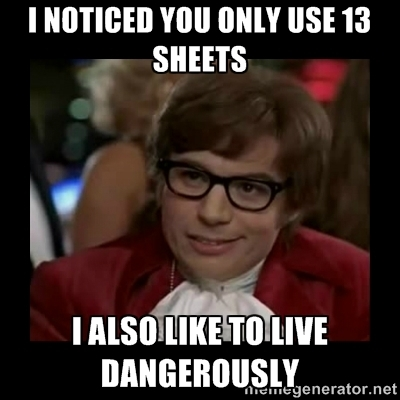
\includegraphics[width=\linewidth]{dangerously.jpg}
\end{center}
\end{multicols}
\end{document}
